\pagebreak
\addcontentsline{toc}{chapter}{Simulado 2}

\num{1} Leia o trecho de um texto.

\begin{quote}
{[}...{]}

D. CARLOTA – Não sei nada; sou uma tagarela, que o senhor obrigou a
dar por paus e por pedras; mas, como é a última vez que nos vemos, não
importa. Agora, passe bem.

CAVALCANTE: Adeus, D. Carlota!

D. CARLOTA: Adeus, doutor!

CAVALCANTE: Adeus. (Dá um passo para a porta do fundo.) Talvez eu vá a
Atenas; não fuja se me vir vestido de frade.

{[}...{]}.

\fonte{Joaquim Maria Machado de Assis. \emph{Não consultes médico}.
Disponível em:
\emph{https://machado.mec.gov.br/obra-completa-lista/item/download/66\_390921fb4791464b4885563dc04a042c}.
Acesso em: 26 fev. 2023.}
\end{quote}

Nesse trecho de texto dramático, a ação a ser desempenhada pelo ator é descrita
no trecho

\begin{minipage}{.5\textwidth}
\begin{escolha}
\item “Adeus, doutor!”

\item “Talvez eu vá a Atenas;”

\item “(Dá um passo para a porta do fundo.)”

\item “Agora, passe bem.”
\end{escolha}
\end{minipage}
\sidetext{SAEB: Identificar as marcas de organização de textos dramáticos. BNCC:
EF35LP24 – Identificar funções do texto dramático (escrito para ser
encenado) e sua organização por meio de diálogos entre personagens e
marcadores das falas das personagens e de cena.}

\num{2} Leia o trecho de um texto.

\begin{quote}
{[}...{]} Em casa, ficaram querendo bem a Escobar; a mesma prima
Justina achou que era um moço muito apreciável, apesar...

– Apesar de quê? perguntou-lhe José Dias, vendo que ela não acabava a frase.

Não teve resposta, nem podia tê-la; prima Justina provavelmente não viu
defeito claro ou importante no nosso hóspede; {[}...{]}.

\fonte{Joaquim Maria Machado de Assis. \emph{Dom Casmurro.}
Disponível em:
\emph{https://machado.mec.gov.br/obra-completa-lista/item/download/13\_7101e1a36cda79f6c97341757dcc4d04}.
Acesso em: 26 fev. 2023.}
\end{quote}

O trecho reproduzido acima apresenta o verbo de enunciação

\begin{minipage}{.5\textwidth}
\begin{escolha}
\item “perguntar”.

\item “ficar”.

\item “ver”.

\item “poder”.
\end{escolha}
\end{minipage}
\sidetext{SAEB: Analisar os efeitos de sentido de verbos de enunciação. BNCC:
EF05LP10 – Ler e compreender, com autonomia, anedotas, piadas e cartuns,
dentre outros gêneros do campo da vida cotidiana, de acordo com as
convenções do gênero e considerando a situação comunicativa e a
finalidade do texto.}

\num{3} Leia o texto.

\begin{quote}
A enfermeira diz ao médico:
– Tem um homem invisível na sala de espera.
O médico responde:
– Diga a ele que não posso vê-lo agora.

\fonte{Domínio público.}
\end{quote}

Os verbos de enunciação presentes nesse texto relacionam-se de modo que o segundo indica que

\begin{escolha}
\item a enfermeira havia feito uma pergunta.

\item a enfermeira ficou sem resposta.

\item o médico ficou nervoso com a fala da enfermeira.

\item o médico referia-se ao que lhe foi dito.
\end{escolha}

\coment{SAEB: Analisar os efeitos de sentido de verbos de enunciação. BNCC:
EF05LP10 – Ler e compreender, com autonomia, anedotas, piadas e cartuns,
dentre outros gêneros do campo da vida cotidiana, de acordo com as
convenções do gênero e considerando a situação comunicativa e a
finalidade do texto.}

\num{4} Leia os trechos.

\begin{quote}
{[}...{]} Quis tapar-lhe a boca. José Dias viu no meu rosto algum
sinal diferente da expressão habitual, e perguntou-me com interesse:

– Que é, Bentinho?

{[}...{]}

\fonte{Joaquim Maria Machado de Assis. \emph{Dom Casmurro.}
Disponível em:
\emph{https://machado.mec.gov.br/obra-completa-lista/item/download/13\_7101e1a36cda79f6c97341757dcc4d04}.
Acesso em: 26 fev. 2023.}
\end{quote}


\begin{quote}
José Dias (olhando com interesse): Que é, Bentinho?

\fonte{Texto adaptado para este material.}
\end{quote}

A partir da comparação entre os dois trechos, pode-se dizer que a
principal diferença entre o texto narrativo e o texto dramático reside

\begin{minipage}{.5\textwidth}
\begin{escolha}
\item no uso de personagens.

\item na temática explorada.

\item na presença de um narrador.

\item no tipo de linguagem explorado.
\end{escolha}
\end{minipage}
\sidetext{SAEB: Reconhecer diferentes gêneros textuais. BNCC: EF35LP29 -
Identificar, em narrativas, cenário, personagem central, conflito
gerador, resolução e o ponto de vista com base no qual histórias são
narradas, diferenciando narrativas em primeira e terceira pessoas.}

\num{5} Leia o texto.

\begin{quote}
\textbf{Superlaboratório Sirius atrai atenção de cientistas da
Argentina, Grã-Bretanha, Alemanha e EUA}

Acelerador de partículas em Campinas (SP) recebeu propostas de
pesquisa de diversas instituições brasileiras e internacionais.
Trabalhos selecionados serão agendados a partir de março.

{[}...{]} o Sirius surge como uma alternativa, já que a máquina é
mundialmente \textbf{competitiva}, possibilita diferentes tipos de
análise com qualidade e com rapidez” {[}...{]}.

\fonte{Fernando Evans. G1. Superlaboratório Sirius atrai atenção de cientistas da Argentina, Grã-Bretanha, Alemanha e EUA. Disponível em:
\emph{https://g1.globo.com/sp/campinas-regiao/noticia/2023/02/17/superlaboratorio-sirius-atrai-atencao-de-cientistas-da-argentina-gra-bretanha-alemanha-e-eua.ghtml}.
Acesso em: 26 fev. 2023.}
\end{quote}

O adjetivo destacado revela, acerca do laboratório, uma visão

\begin{minipage}{.5\textwidth}
\begin{escolha}
\item duvidosa.

\item neutra.

\item positiva.

\item negativa.
\end{escolha}
\end{minipage}
\sidetext{SAEB: Analisar os efeitos de sentido decorrentes do uso dos adjetivos.
Não há correspondência com a BNCC do quinto ano.}

\num{6} Analise esta tabela.


\begin{tabular}{|ll|}
\hline
\multicolumn{2}{|c|}{\begin{tabular}[c]{@{}c@{}}Número de alunos matriculados nos Anos Iniciais\\ Município de Fortaleza (CE)\end{tabular}} \\ \hline
\multicolumn{1}{|l|}{1º ano} & 18.221 \\ \hline
\multicolumn{1}{|l|}{2º ano} & 17.850 \\ \hline
\multicolumn{1}{|l|}{3º ano} & 18.435 \\ \hline
\multicolumn{1}{|l|}{4º ano} & 19.513 \\ \hline
\multicolumn{1}{|l|}{5º ano} & 20.103 \\ \hline
\end{tabular}

\fonte{Fonte de pesquisa: QEdu, 2021. Disponível em: \emph{https://qedu.org.br/municipio/2304400-fortaleza/censo-escolar}. Acesso em: 28 mar. 2023.}

Segundo a tabela, o ano escolar, entre os dos Anos Iniciais, com menos matriculados é o

\begin{minipage}{.5\textwidth}
\begin{escolha}
\item 1º ano.

\item 2º ano.

\item 3º ano.

\item 4º ano.
\end{escolha}
\end{minipage}
\sidetext{SAEB: Analisar informações apresentadas em gráficos, infográficos ou
tabelas. BNCC: EF05LP23 – Comparar informações apresentadas em gráficos
ou tabelas.}

\num{7} Leia o texto a seguir e responda à pergunta:

\begin{quote}
O mini-helicóptero Ingenuity, da Nasa, entrou para o “Guinness World
Records” com o voo mais longo realizado na superfície marciana.

{[}...{]}

O Ingenuity, que se assemelha a um drone, pesa 1,8kg e chegou a Marte
dobrado e acoplado à parte inferior do Perseverance, robô da Nasa que
pousou no planeta em fevereiro de 2021.

{[}...{]}

“Temos confiança de que podemos contar com o Perseverance para trazer
as amostras de volta e adicionamos os helicópteros como uma espécie de
plano B”, disse Gramling.

{[}...{]}.

\fonte{G1. Helicóptero da Nasa entra para o “Guinness World Records” com o voo mais longo em Marte. Disponível em: \emph{https://g1.globo.com/ciencia/noticia/2023/02/14/helicoptero-da-nasa-entra-para-o-guinness-world-records-com-o-voo-mais-longo-em-marte.ghtml}. Acesso em: 26 fev. 2023.}
\end{quote}

No texto, é uma opinião que

\begin{escolha}
\item o Perseverance vai trazer para a Terra amostras de Marte.

\item o Ingenuity realizou o voo mais longo na superfície de Marte.

\item o Ingenuity é um mini-helicóptero da Nasa.

\item o robô Perseverance pousou em Marte no ano de 2021.
\end{escolha}

\coment{SAEB: Distinguir fatos de opiniões em textos. BNCC: EF05LP16 – Comparar
informações sobre um mesmo fato veiculadas em diferentes mídias e
concluir sobre qual é mais confiável e por quê.}

\num{8}  Leia o texto.

O instrumento musical afoxé é composto de uma cabaça coberta por uma
rede formada por sementes, miçangas ou contas.

\begin{figure}[htpb!]
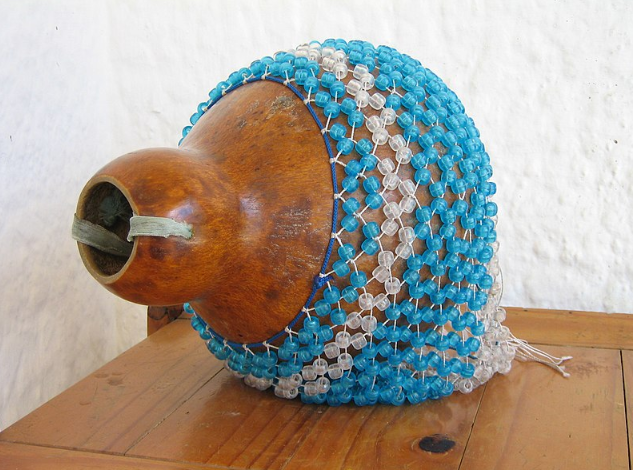
\includegraphics[width=\textwidth]{./imgs/art33.png}
\end{figure}

O som desse instrumento é
produzido quando se gira a rede em um sentido e a base do instrumento (a
cabaça) no sentido oposto.

Assinale a alternativa que corresponde à forma como o som do afoxé é
produzido.

\begin{escolha}
\item
  Produz som pela vibração do instrumento.
\item
  Produz som pela vibração de cordas.
\item
  Produz som pela vibração de uma membrana esticada em algum suporte.
\item
  Produz som pela vibração do ar no seu interior.
\end{escolha}

\coment{SAEB: Identificar as características de instrumentos musicais
variados, bem como o potencial musical do corpo humano.}

\num{9}  Leia o texto.

Arte afro-brasileira é uma manifestação que retoma a estética e religiosidade africanas tradicionais, além dos contextos socioculturais do negro no Brasil.

Assinale a alternativa que contém um exemplo de arte afro-brasileira.

\begin{figure}[htpb!]
\acima{a)}
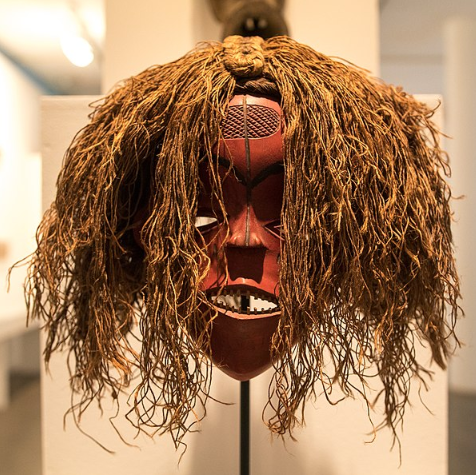
\includegraphics[width=.5\textwidth]{./imgs/art34a.png}
\caption{Máscara dos yakas, grupo étnico de Angola. Museu Afro Brasil.}
\end{figure}
\begin{figure}[htpb!]
\acima{b)}
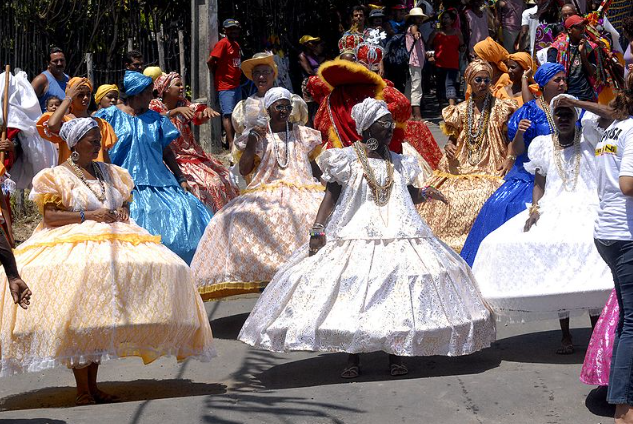
\includegraphics[width=.5\textwidth]{./imgs/art34b.png}
\caption{Cortejo de maracatu. Recife, Brasil.}
\end{figure}

\begin{figure}[htpb!]
\acima{c)}
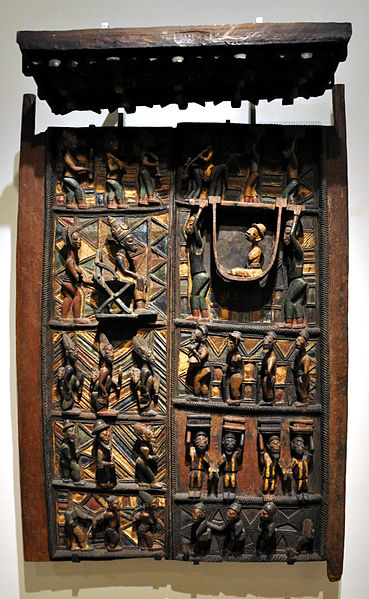
\includegraphics[width=.5\textwidth]{./imgs/art34c.jpg}
\caption{Painel de porta (1910-1914), povo iorubá, Nigéria, África.}
\end{figure}
\begin{figure}[htpb!]
\acima{d)}
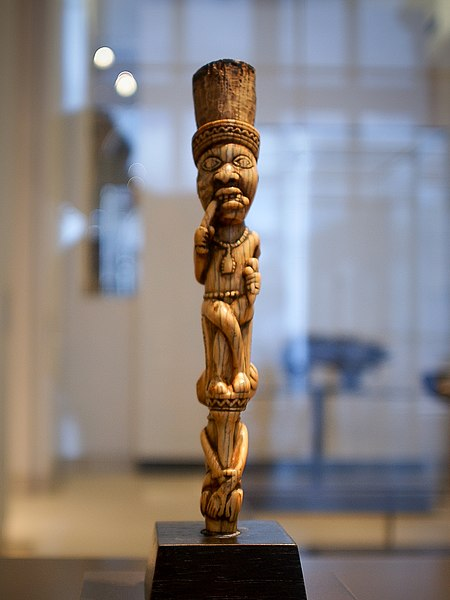
\includegraphics[width=.5\textwidth]{./imgs/art34d.jpg}
\caption{Escultura yumbe, da República Democrática do Congo, África.}
\end{figure}

\coment{SAEB: Reconhecer a influência de distintas matrizes estéticas e
culturais nas manifestações das artes visuais, dança, música e teatro na
cultura brasileira.
BNCC: EF15AR03 – Reconhecer e analisar a influência de distintas
matrizes estéticas e culturais das artes visuais nas manifestações
artísticas das culturas locais, regionais e nacionais.}

\num{10} Assinale a alternativa que apresenta movimento corporal próprio das danças do hip-hop.

\begin{figure}[htpb!]
\acima{a)}
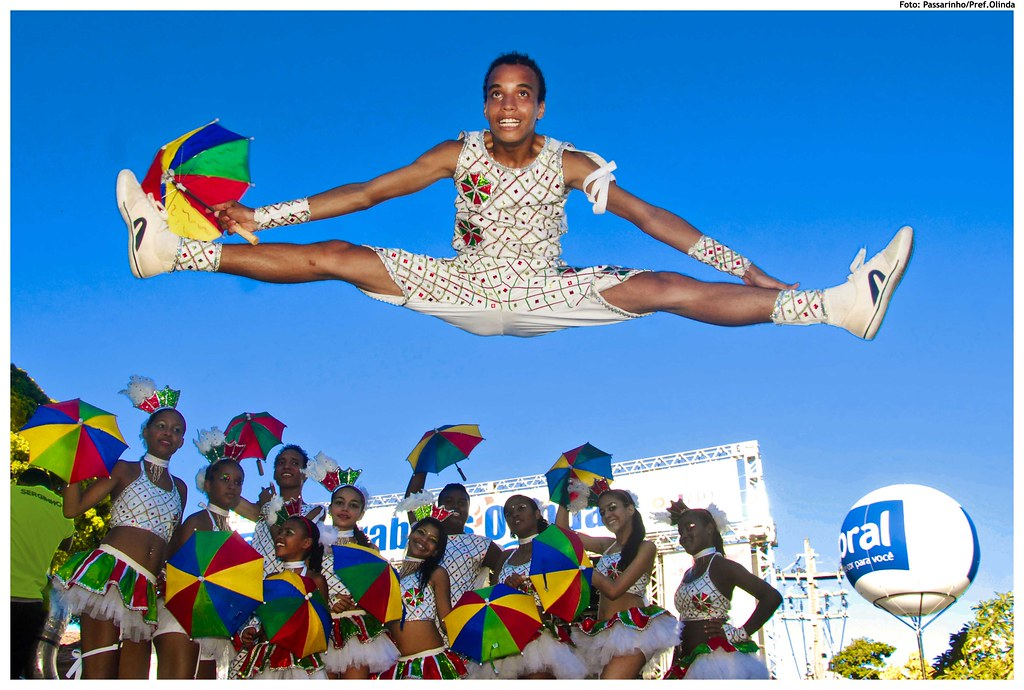
\includegraphics[width=.5\textwidth]{./imgs/art35a.jpg}
\end{figure}
\begin{figure}[htpb!]
\acima{b)}
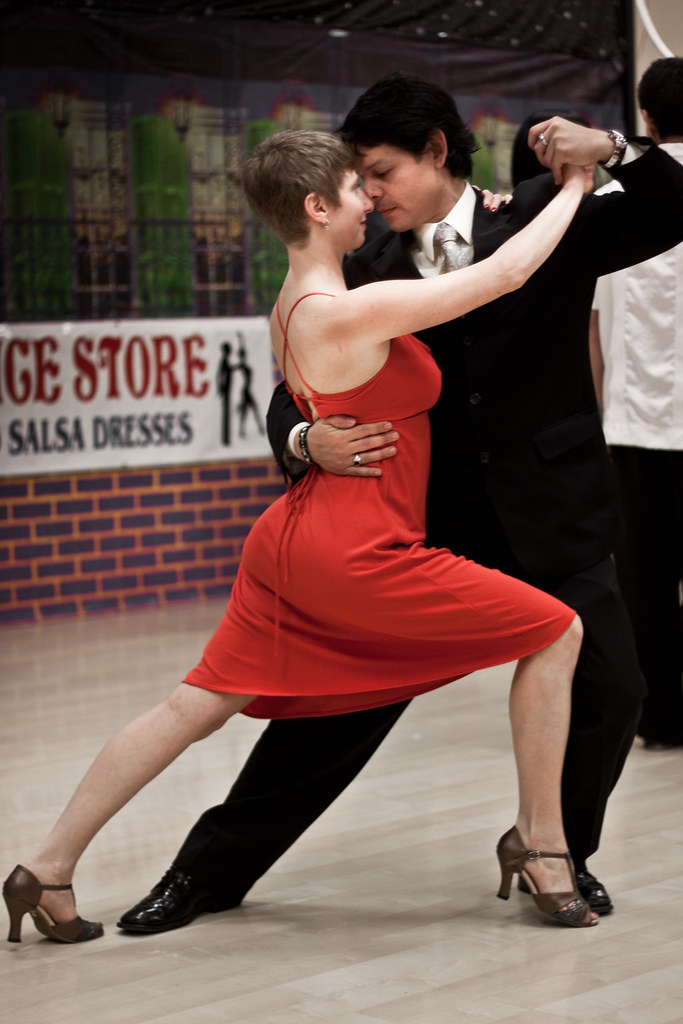
\includegraphics[width=.5\textwidth]{./imgs/art35b.jpg}
\end{figure}

\begin{figure}[htpb!]
\acima{c)}
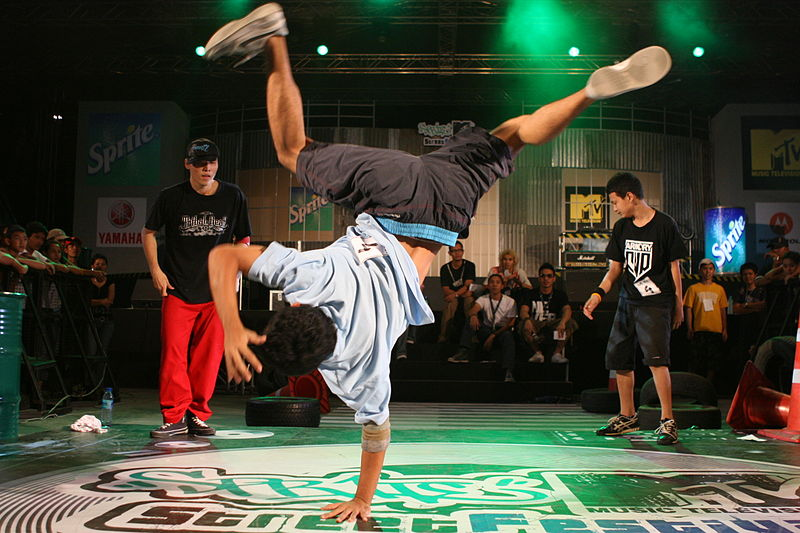
\includegraphics[width=.5\textwidth]{./imgs/art35c.jpg}
\end{figure}
\begin{figure}[htpb!]
\acima{d)}
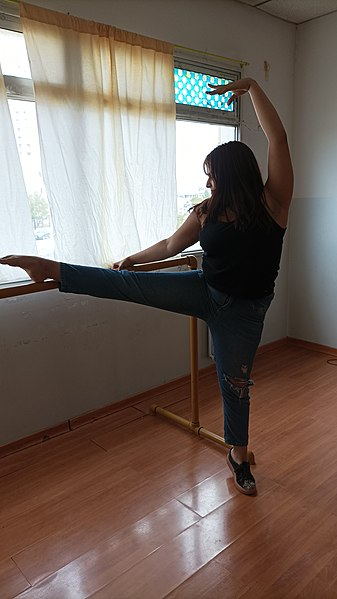
\includegraphics[width=.5\textwidth]{./imgs/art35d.jpg}
\end{figure}

\coment{SAEB: Analisar relações entre as partes corporais e seu todo na
estética da dança.}


%\begin{figure}[htpb!]
%\vspace*{-3cm}
%\hspace*{-2.5cm}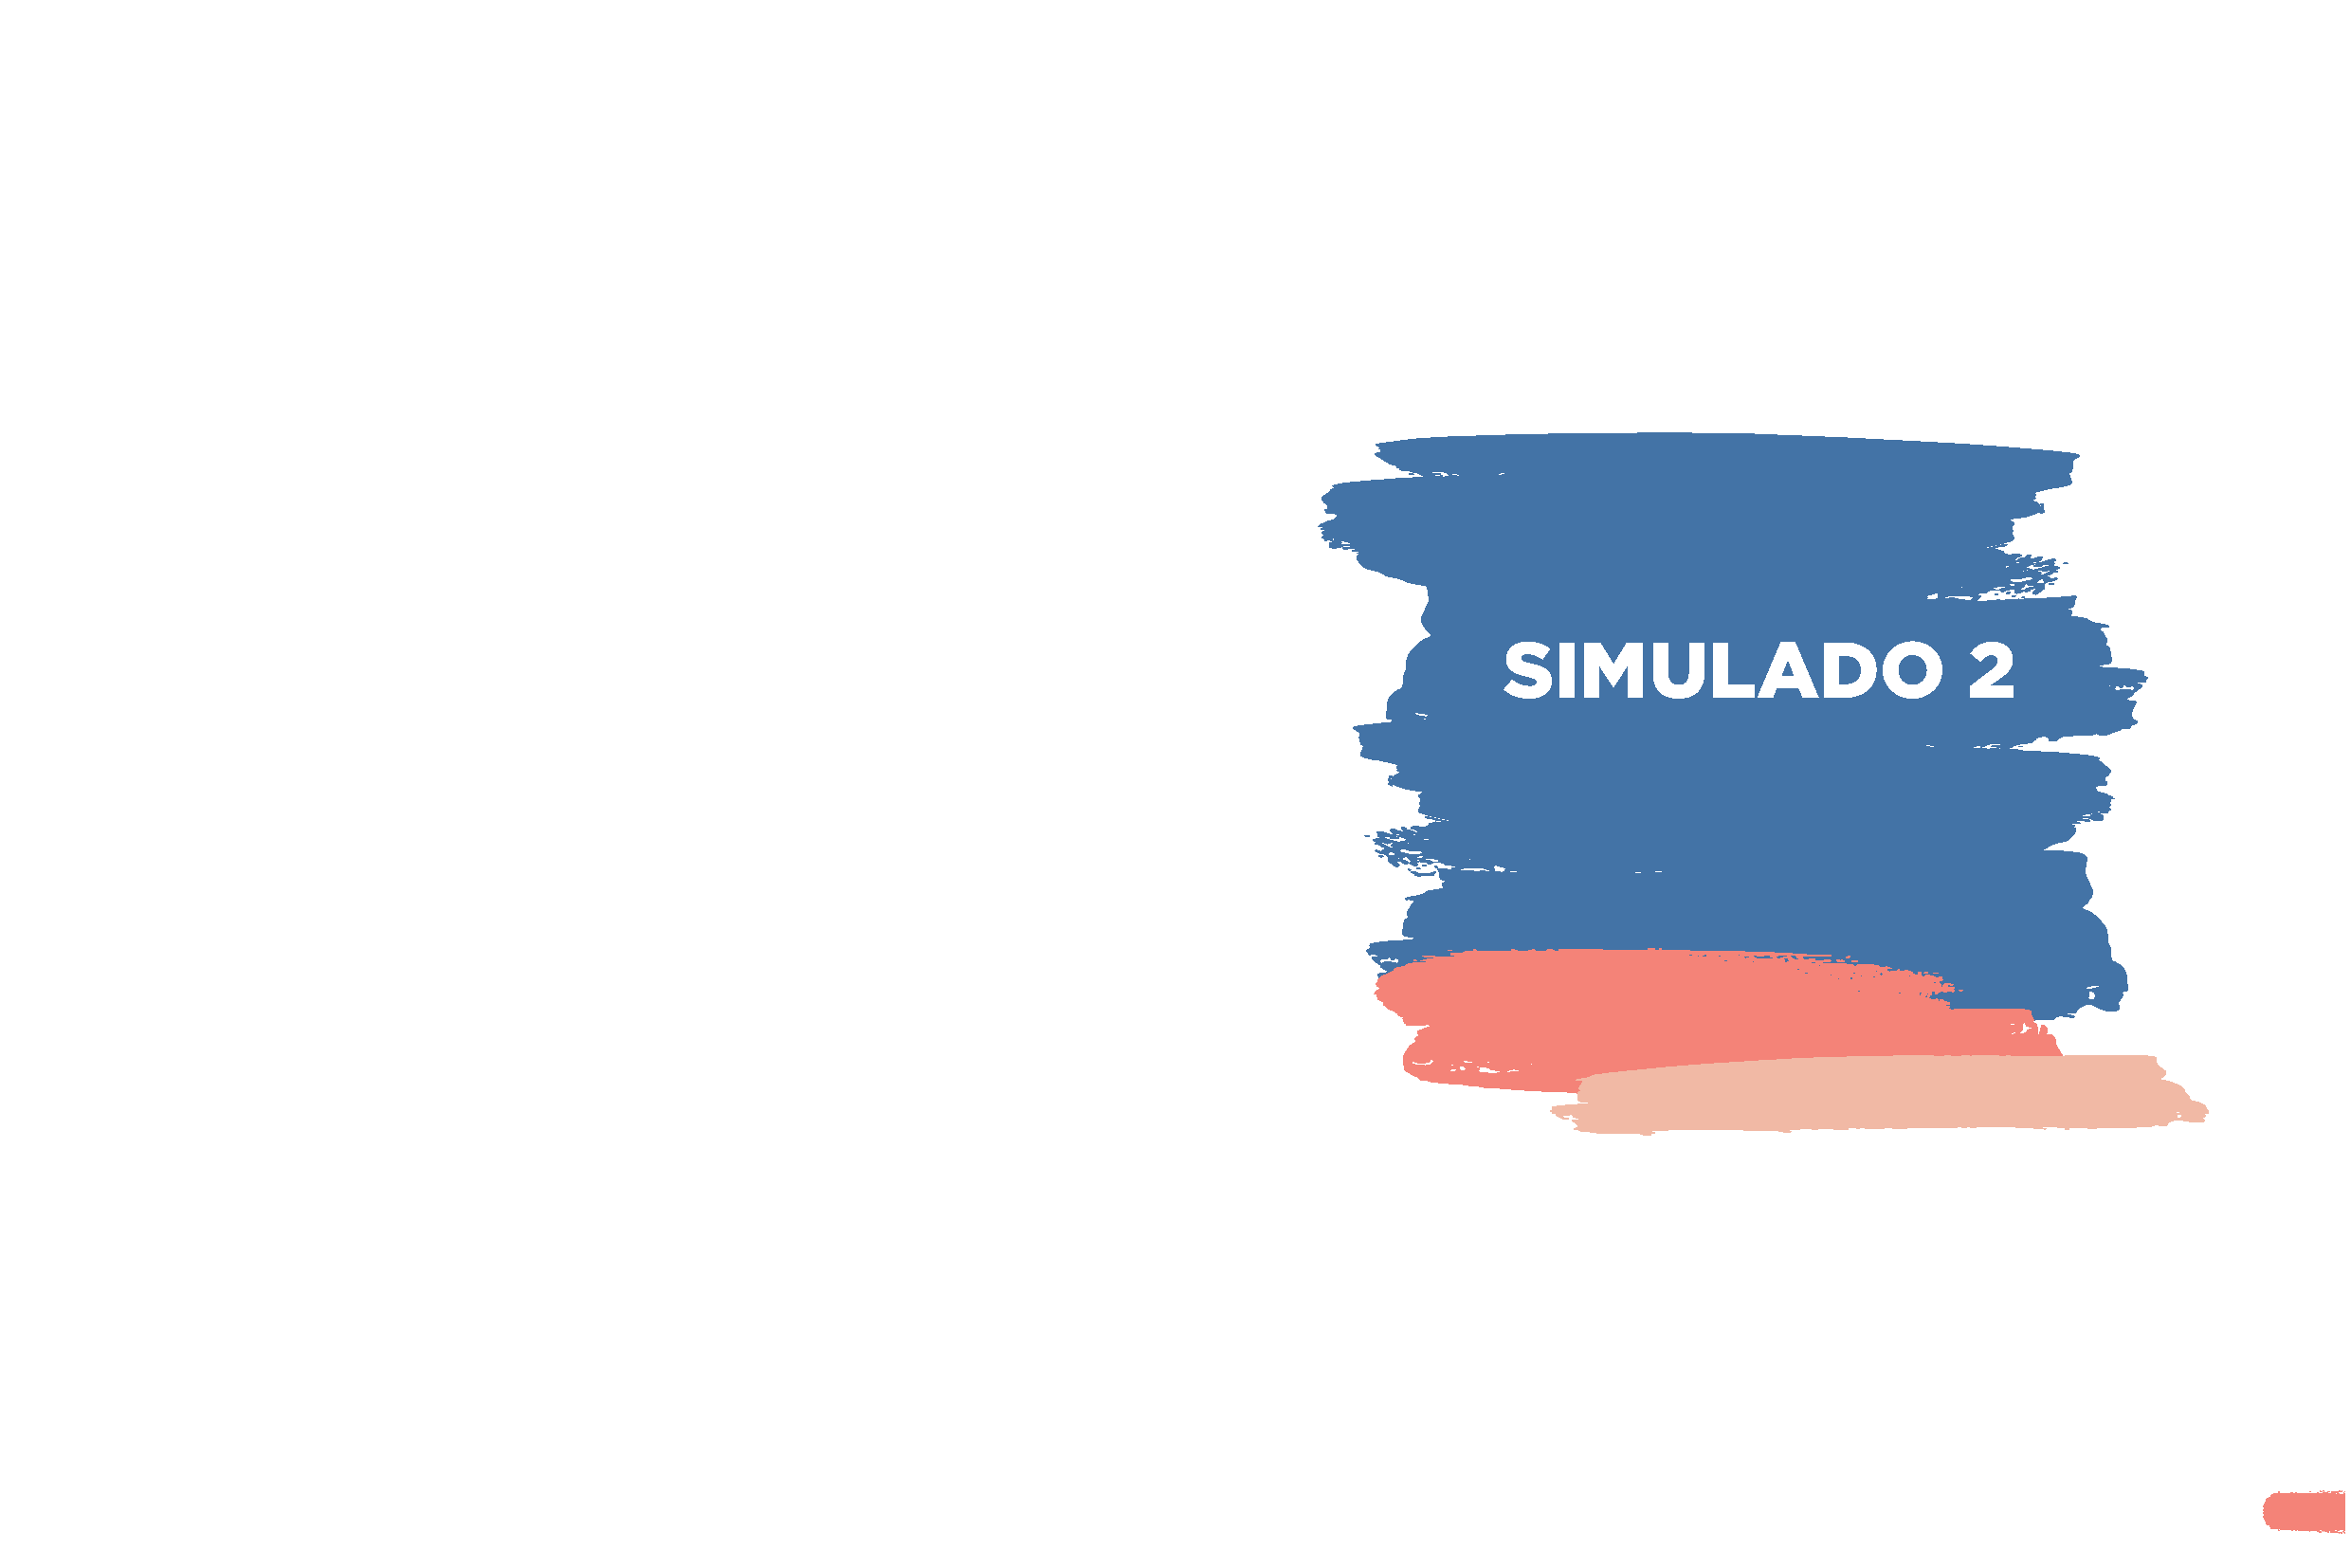
\includegraphics[scale=1]{../watermarks/2simulado5ano.pdf}
%\end{figure}
%
%\newwatermark[pagex={61,63}]{\vspace{2.5cm}\hspace*{8cm}\includegraphics[scale=1]{../watermarks/%bgsim5anoimpar.pdf}}
%\newwatermark[pagex={62}]{\vspace{2.5cm}\hspace*{7.8cm}\includegraphics[scale=1]{../watermarks/%bgsim5anopar.pdf}}
%
%\pagebreak
%\movetooddpage
%\markboth{Simulado 2}{}

\num{11} A Cetesb iniciou nesta quinta-feira, dia 16/04, a operação da nova
estação de monitoramento da qualidade do ar, instalada na escola de
educação infantil Prof. Zeferino Vaz, em Campinas. A unidade foi
adquirida com recursos de compensação ambiental do Aeroporto
Internacional de Viracopos, em função das obras de ampliação. {[}\ldots{}{]} A estação
vai avaliar a qualidade do ar da cidade, levando em consideração os
possíveis impactos de Viracopos, das rodovias Anhanguera, Bandeirantes e
Santos Dumont, bem como o conhecimento dos processos de transporte de
poluentes oriundos de outras regiões. {[}\ldots{}{]}

\fonte{Governo do estado de São Paulo. Secretaria de Meio Ambiente, Infraestrutura e Logística. Disponível em:
\emph{https://www.infraestruturameioambiente.sp.gov.br/2015/04/cetesb-inicia-hoje-operacao-da-nova-estacao-de-monitoramento-do-ar-de-campinas/}.
Acesso em: 23 fev. 2023.}

A medida no município de Campinas, em São Paulo, é
importante para

\begin{escolha}
\item entender o impacto dos transportes na cidade.

\item diminuir a circulação de produtos na região.

\item avaliar os resultados de políticas ambientais.

\item melhorar a qualidade da educação nas escolas.
\end{escolha}

\coment{BNCC: EF05GE12 - Identificar órgãos do poder público e canais de participação
social responsáveis por buscar soluções para a melhoria da qualidade de
vida (em áreas como meio ambiente, mobilidade, moradia e direito à
cidade) e discutir as propostas implementadas por esses órgãos que
afetam a comunidade em que vive.}

\num{12} O Brasil é dividido em cinco regiões. Identifique cada uma conforme sua numeração no mapa abaixo:


\begin{escolha}
\item 1 - Nordeste, 2 - Centro-Oeste, 3 - Sudeste, 4 - Sul, 5 - Norte.

\item 1 - Norte, 2 - Centro-Oeste, 3 - Sul, 4 - Sudeste, 5 - Nordeste.

\item 1 - Nordeste, 2 - Sul, 3 - Norte, 4 - Centro-Oeste, 5 - Sudeste.

\item 1 - Norte, 2 - Sul, 3 - Centro-Oeste, 4 Sudeste, 5 - Nordeste.
\end{escolha}

\begin{figure}[htpb!]
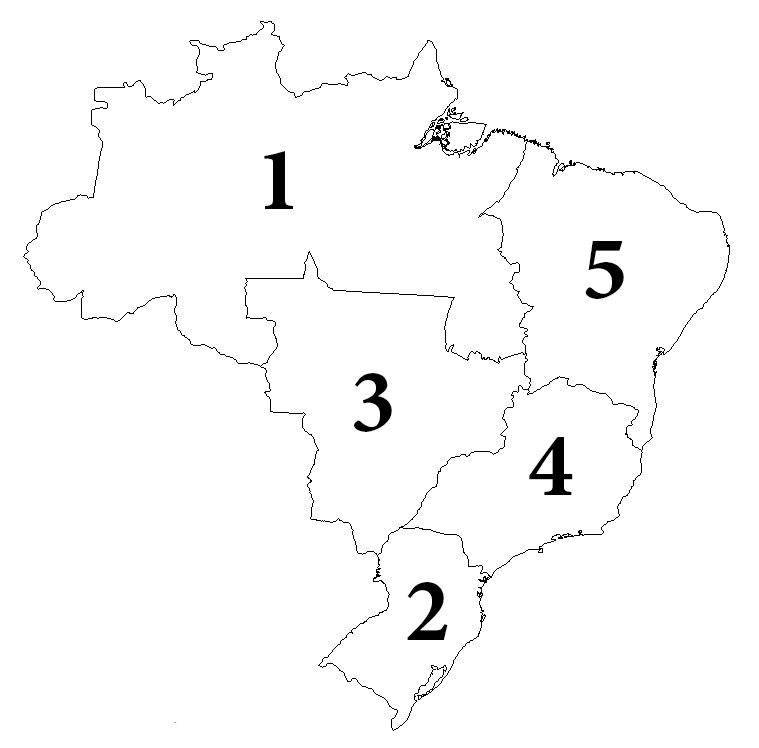
\includegraphics[width=\textwidth]{../ilustracoes/CHU5/SAEB_5ANO_CHU_FIGURA1.png}
\end{figure}

\coment{BNCC: EF05HI02 - Identificar os mecanismos de organização do
poder político com vistas à compreensão da ideia de Estado e/ou de
outras formas de ordenação social.}

\num{13}

\begin{quote}
Entre 2003 e 2013 diversas cidades brasileiras viram protestos sobre a
gratuidade do transporte coletivo. {[}\ldots{}{]} Em 2013 o aumento da passagem em São
Paulo levou milhares de manifestantes às ruas. O Movimento Passe Livre
foi um dos grupos responsáveis pela divulgação e pela extensão que os
protestos ganharam. {[}\ldots{}{]} Atualmente, no Brasil, diversas cidades adotam algum
tipo de isenção ou redução da tarifa principalmente para idosos,
deficientes ou estudantes. Algumas até aderiram à gratuidade integral,
sendo Volta Redonda (RJ), com 257.803 habitantes, e Maricá (RJ) 143.111
habitantes, as representantes mais populosas. {[}\ldots{}{]}

\fonte{Estadão. Passe Livre: conheça a história do movimento. Disponível em:
\emph{https://summitmobilidade.estadao.com.br/compartilhando-o-caminho/passe-livre-conheca-a-historia-do-movimento/}.
Acesso em: 23 fev. 2023.}
\end{quote}

\noindent{}O Movimento Passe Livre, segundo o trecho, reivindicava

\begin{escolha}
\item ajudas do governo na compra de carros particulares.

\item melhorias das condições de trabalho dos motoristas.

\item utilização do transporte público de maneira gratuita.

\item reformas dos asfaltos das grandes metrópoles do país.
\end{escolha}

\coment{BNCC: EF05HI05 - Associar o conceito de cidadania à conquista
de direitos dos povos e das sociedades, compreendendo-o como conquista
histórica.}

\num{14}

\begin{quote}
Campo Grande é, historicamente, a região do Rio de Janeiro com maior
potencial de crescimento, por várias razões. Como está situado em região de limite do município, o lugar teve sua planície atravessada desde muito tempo. Além disso, lá há muitas reservas de água e muitas pessoas com interesses empreendedores. Atualmente, a economia local é composta por cerca de 3.700 estabelecimentos. 
\end{quote}

Segundo o texto, o bairro Campo Grande, no Rio de Janeiro, tem potencial
de crescimento por causa de sua

\begin{escolha}
\item boa localização e interesse econômico.

\item qualidade educacional e beleza natural.

\item atração turística e importância histórica.

\item riqueza mineral e produção gastronômica.
\end{escolha}

\coment{BNCC: EF05HI0 - Identificar os processos de
formação das culturas e dos povos, relacionando-os com o espaço
geográfico ocupado.}

\num{15}

\begin{quote}
\textbf{Ingredientes para receita de Hambúrguer:}\\
200 gramas de carne moída\\
1 tomate\\
100 gramas de alface\\
1 cebola\\
1 pão
\end{quote}

\noindent{}De quais setores de trabalho precisamos para conseguir os ingredientes
para preparar uma receita de hambúrguer em casa?

\begin{minipage}{0.5\textwidth}
\begin{escolha}
\item agricultura e pecuária.

\item agricultura e turismo.

\item pecuária e mineração.

\item pecuária e turismo.
\end{escolha}
\end{minipage}
\sidetext{BNCC: EF05GE05 - Identificar e comparar as mudanças dos tipos de trabalho
e desenvolvimento tecnológico na agropecuária, na indústria, no comércio
e nos serviços.}